Analisis sistem terdiri dari gambaran umum sistem yang dapat dilihat pada Gambar \ref{fig:gambaran-umum}, deskripsi sistem, dan diagram alir sistem. Gambaran umum sistem menjelaskan secara singkat tentang sistem yang akan dibangun. Deskripsi sistem menjelaskan tentang sistem yang akan dibangun secara rinci. Diagram alir sistem menjelaskan tentang alur kerja sistem yang akan dibangun.

\begin{figure}[H]
    \centering
    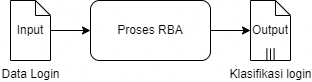
\includegraphics[width=0.6\textwidth]{BAB_TESIS/IMAGES/gambaran-umum.png}
    \caption{Gambaran Umum Sistem}
    \label{fig:gambaran-umum}
\end{figure}

